%% ----------------------------------------------------------------
%% Thesis.tex -- MAIN FILE (the one that you compile with LaTeX)
%% ---------------------------------------------------------------- 

% Set up the document
\documentclass[a4paper, 11pt, oneside]{Thesis}  % Use the "Thesis" style, based on the ECS Thesis style by Steve Gunn
\graphicspath{Figures/}  % Location of the graphics files (set up for graphics to be in PDF format)

\usepackage[utf8]{inputenc}
\usepackage[printonlyused,withpage]{acronym}
% Include any extra LaTeX packages required
\usepackage[square, numbers, comma, sort&compress]{natbib}  % Use the "Natbib" style for the references in the Bibliography
\usepackage{verbatim}  % Needed for the "comment" environment to make LaTeX comments
\usepackage{vector}  % Allows "\bvec{}" and "\buvec{}" for "blackboard" style bold vectors in maths
\hypersetup{urlcolor=black, citecolor=black, linkcolor=black}  % Colours hyperlinks in blue, but this can be distracting if there are many links.


% tikz and flowchart
\usepackage{tikz}
\usetikzlibrary{shapes.geometric, arrows}

% define color
\definecolor{olivegreen}{RGB}{34,139,34}
\definecolor{darkorange}{RGB}{255,140,0}


%% ----------------------------------------------------------------
\begin{document}
\frontmatter      % Begin Roman style (i, ii, iii, iv...) page numbering


%%%%%%%%% Title page from scratch %%%%%%%%
\begin{titlepage}
    \centering
    \vfill
    {\bfseries\LARGE
    	\vskip1cm
        Undergraduate senior project \\
        \vskip1cm
    }    
    
\includegraphics[width=6cm]{img/mahidol} % also works with logo.pdf
    \noindent\rule{\textwidth}{1.0pt}
    {\bfseries\huge
    	\vskip0.2cm
        Study of cosmic-ray spectrum using gamma-ray data from \textit{Fermi} Large Area Telescope
        \vskip0.2cm
    }    
    \noindent\rule{\textwidth}{1.0pt}
    {\bfseries\LARGE
    	\vskip1cm
        Patomporn Payoungkhamdee 5705108 \\
        \vskip0.4cm
        Department of Physics, Faculty of Sciences \\
        \vskip0.2cm
        Mahidol University
    }    
    \vfill
    \vfill
\end{titlepage}
%%%%%%%% end title from scratch %%%%%%%%%%%


% Set up the Title Page
\title  {Study of cosmic-ray spectrum using gamma-ray data from \textit{Fermi} Large Area Telescope}
\authors  {\texorpdfstring
            {\href{patomporn.pay@gmail.com}{Patomporn Payoungkhamdee}}
            {Patomporn Payoungkhamdee}
            }
\addresses  {\groupname\\\deptname\\\univname}  % Do not change this here, instead these must be set in the "Thesis.cls" file, please look through it instead
\date       {\today}
\subject    {}
\keywords   {}

% \maketitle
%% ----------------------------------------------------------------

\setstretch{1.3}  % It is better to have smaller font and larger line spacing than the other way round

% Define the page headers using the FancyHdr package and set up for one-sided printing
\fancyhead{}  % Clears all page headers and footers
\rhead{\thepage}  % Sets the right side header to show the page number
\lhead{}  % Clears the left side page header

\pagestyle{fancy}  % Finally, use the "fancy" page style to implement the FancyHdr headers
%% ----------------------------------------------------------------
%%      Declaration
%% ----------------------------------------------------------------
% Declaration Page required for the Thesis, your institution may give you a different text to place here
% \Declaration{

% \addtocontents{toc}{\vspace{1em}}  % Add a gap in the Contents, for aesthetics

% I, AUTHOR NAME, declare that this thesis titled, `THESIS TITLE' and the work presented in it are my own. I confirm that:

% \begin{itemize} 
% \item[\tiny{$\blacksquare$}] This work was done wholly or mainly while in candidature for a research degree at this University.
 
% \item[\tiny{$\blacksquare$}] Where any part of this thesis has previously been submitted for a degree or any other qualification at this University or any other institution, this has been clearly stated.
 
% \item[\tiny{$\blacksquare$}] Where I have consulted the published work of others, this is always clearly attributed.
 
% \item[\tiny{$\blacksquare$}] Where I have quoted from the work of others, the source is always given. With the exception of such quotations, this thesis is entirely my own work.
 
% \item[\tiny{$\blacksquare$}] I have acknowledged all main sources of help.
 
% \item[\tiny{$\blacksquare$}] Where the thesis is based on work done by myself jointly with others, I have made clear exactly what was done by others and what I have contributed myself.
% \\
% \end{itemize}
 
 
% Signed:\\
% \rule[1em]{25em}{0.5pt}  % This prints a line for the signature
 
% Date:\\
% \rule[1em]{25em}{0.5pt}  % This prints a line to write the date
% }
% \clearpage  % Declaration ended, now start a new page

%% ----------------------------------------------------------------
% The "Funny Quote Page"
\pagestyle{empty}  % No headers or footers for the following pages

\null\vfill
% Now comes the "Funny Quote", written in italics
“We are trying to prove ourselves wrong as quickly as possible, because only in that way can we find progress.” 
\begin{flushright}
Richard Feynman
\end{flushright}

\vfill\vfill\vfill\vfill\vfill\vfill\null
\clearpage  % Funny Quote page ended, start a new page
%% ----------------------------------------------------------------

% The Abstract Page
\addtotoc{Abstract}  % Add the "Abstract" page entry to the Contents
\abstract{
\addtocontents{toc}{\vspace{1em}}  % Add a gap in the Contents, for aesthetics
Cosmic rays (CRs) are high-energy particles propagating in space. They are mainly constituted by protons and the energy spectrum is well described by a power law.
Recent measurements by PAMELA and AMS-02 indicate an abrupt change of the CR proton spectral index at about 300 GeV.
When protons interact with the Earth's upper atmosphere, $\gamma$-rays can be produced and detected by space-based detectors. We use the Earth Limb $\gamma$-ray data collected by the \textit{Fermi} Large Area Telescope (LAT) along with proton-air interaction models to determine the CR proton spectral indices that best fit the $\gamma$-ray data. 
\\ \textbf{Keyword:} Cosmic rays, gamma rays, \textit{Fermi}-LAT
% Cosmic rays (CRs) are high energy particles in space, mainly protons, for which the spectrum is well described by a power law. Recent measurements from PAMELA and AMS-02 indicate an abrupt change of the CR proton spectral index at $\sim$300 GeV. When CRs interact with the Earth's upper atmosphere, \acf{gmr} photons can be produced and detected by space-based detectors. We use the Earth's $\gamma$-ray data observed by the \acf{Fermi-LAT} along with proton-air interaction model perform Monte Carlo simulation and determine the CR proton spectral indices that best fit the $\gamma$-ray data.
}

\clearpage  % Abstract ended, start a new page
%% ----------------------------------------------------------------

\setstretch{1.3}  % Reset the line-spacing to 1.3 for body text (if it has changed)

% The Acknowledgements page, for thanking everyone
\acknowledgements{
\addtocontents{toc}{\vspace{1em}}  % Add a gap in the Contents, for aesthetics


I would like to thanks to Dr. Warit Mitthumsiri and Dr. Francesca Spada for their advise and any other supervision.

\par To begin with project I also appreciate Mr. Suttiwat Madlee for any recommendation and revise my program knowledge.
This work also be fulfill the improvement in terms of theory and instrument correction by Prof. Luca Baldini, Dr. Carmelo Sgrò, Mr. Niccolò Di Lalla, Mr. Alberto Manfreda, as well as to people in the Space Physics laboratory at Mahidol University and the Fermi lab at the University of Pisa. 

Last but not least, I would like to to thanks Development and Promotion of Science and Technology Talents Project (DPST) for any finalcial support since I was starting this work. This work was partially supported by the Thailand Research Fund award RTA5980003.
% The acknowledgements and the people to thank go here, don't forget to include your project advisor\ldots

}
\clearpage  % End of the Acknowledgements
%% ----------------------------------------------------------------

\pagestyle{fancy}  %The page style headers have been "empty" all this time, now use the "fancy" headers as defined before to bring them back


%% ----------------------------------------------------------------
\lhead{\emph{Contents}}  % Set the left side page header to "Contents"
\tableofcontents  % Write out the Table of Contents

%% ----------------------------------------------------------------
\lhead{\emph{List of Figures}}  % Set the left side page header to "List if Figures"
\listoffigures  % Write out the List of Figures

%% ----------------------------------------------------------------
\lhead{\emph{List of Tables}}  % Set the left side page header to "List of Tables"
\listoftables  % Write out the List of Tables



\chapter{Abbreviations}
\lhead{\emph{Abbreviations}}
\begin{acronym}[TDMA]

\acro{Fermi-LAT}[\textit{Fermi}-LAT]{\textit{Fermi} Large Area Telescope}
\acro{Pamela}[PAMELA]{Payload for Antimatter Matter Exploration and Light-nuclei Astrophysics}
\acro{CR}[CR]{Cosmic ray}
\acro{gmr}[$\gamma$-ray]{gamma-ray}
\acro{spl}[SPL]{Single power law}
\acro{bpl}[BPL]{Broken power law}
\acro{lrt}[LRT]{Likelihood ratio test}

\end{acronym}

%% ----------------------------------------------------------------
\clearpage  % Start a new page
\lhead{\emph{Physical Constants}}  % Set the left side page header to "Physical Constants"
\listofconstants{lrcl}  % Include a list of Physical Constants (a four column table)
{
% Constant Name & Symbol & = & Constant Value (with units) \\
Speed of Light & $c$& $=$ & $2.997 \times10^{8}\ \mbox{ms}^{-\mbox{s}}$ (exact)\\
Mass of proton & $m_\text{p}$& $=$ & $938.272\ \mbox{MeV/c}^{2}$\\
Mass of Helium atom & $m_\text{He}$& $=$ & $3.727\ \mbox{GeV/c}^{2}$
}

%% ----------------------------------------------------------------
\clearpage  %Start a new page
\lhead{\emph{Symbols}}  % Set the left side page header to "Symbols"
\listofnomenclature{lll}  % Include a list of Symbols (a three column table)
{
% symbol & name & unit \\
$\Omega$ & Solid angle & rad$^2$ \\
$E$ & Energy & GeV \\
$E_k$ & Kinetic energy & GeV \\
$R$ & Rigidity & GV \\
& & \\ % Gap to separate the Roman symbols from the Greek
$\theta_\text{LAT}$ & Azimuth angle from Z-axis of detector plane & $\mbox{rad}$ \\
$\phi_\text{LAT}$ & Angle in +X direction of detector plane & $\mbox{rad}$ \\
$\theta_\text{ZENITH}$ & Angle between event photon and zenith line & $\mbox{rad}$ \\
$\theta_\text{NADIR}$ & Defined from inclination angle relative to zenith direction & $\mbox{rad}$ \\
$\sigma$ & Crossection & $\mbox{mb}$
}
%% ----------------------------------------------------------------
% End of the pre-able, contents and lists of things
% Begin the Dedication page

\setstretch{1.3}  % Return the line spacing back to 1.3

%%% For skipping dedicate page
% \pagestyle{empty}  % Page style needs to be empty for this page
% \dedicatory{Dedicated To my parents}

\addtocontents{toc}{\vspace{2em}}  % Add a gap in the Contents, for aesthetics


%% ----------------------------------------------------------------
\mainmatter	  % Begin normal, numeric (1,2,3...) page numbering
\pagestyle{fancy}  % Return the page headers back to the "fancy" style

% Include the chapters of the thesis, as separate files
% Just uncomment the lines as you write the chapters

\chapter{Introduction}
\lhead{Introduction}

% describe cosmic ray study since past to now just brief
\par Since the study of \acf{CR} has been led by Theodor Wulf who taked electrometer measured \acf{CR} from the ground to higher altitude and much more experiment has confirmed that there is a cosmic ray from outer space which can penetrate to the Earth's surface \cite{HESS,Pacini,Clay}.

% Consequently
\par Consequently, there are many possible phenomena of acceleration mechanism in the space that could produced high energy particles which would be a \acs{CR}. In order to study the characteristic of acceleration mechanism, we could take consider \acs{CR} spectrum which has a unique energy break point of superposition between different phenomena.

In 2011, \acs{Pamela} detecter indicate that there is a break point of proton cosmic ray spectrum around 240 GV \cite{PAMELA}. Furthermore, AMS-02 also found a drastic change of proton CR spectrum at around 336 GV. \cite{AMS-02}
% Early study, and what we gonna do
\par \acs{CR} are mainly compose with proton and 10$\%$ by Helium. Generally, \acf{gmr} could be produced by \acs{CR} collide with Earth's upper atmosphere. In this study, we perform an indirect measurement of proton spectrum from \acs{gmr} data which collected by \acf{Fermi-LAT} to find best fit incident proton spectrum that best fit to \acs{gmr} spectrum.
 % Introduction

\chapter{Background knowledge}
\lhead{Background knowledge}

%==========================
%    Cosmic ray
%==========================
\section{Cosmic rays}
\begin{figure}[h!]
  \centering
    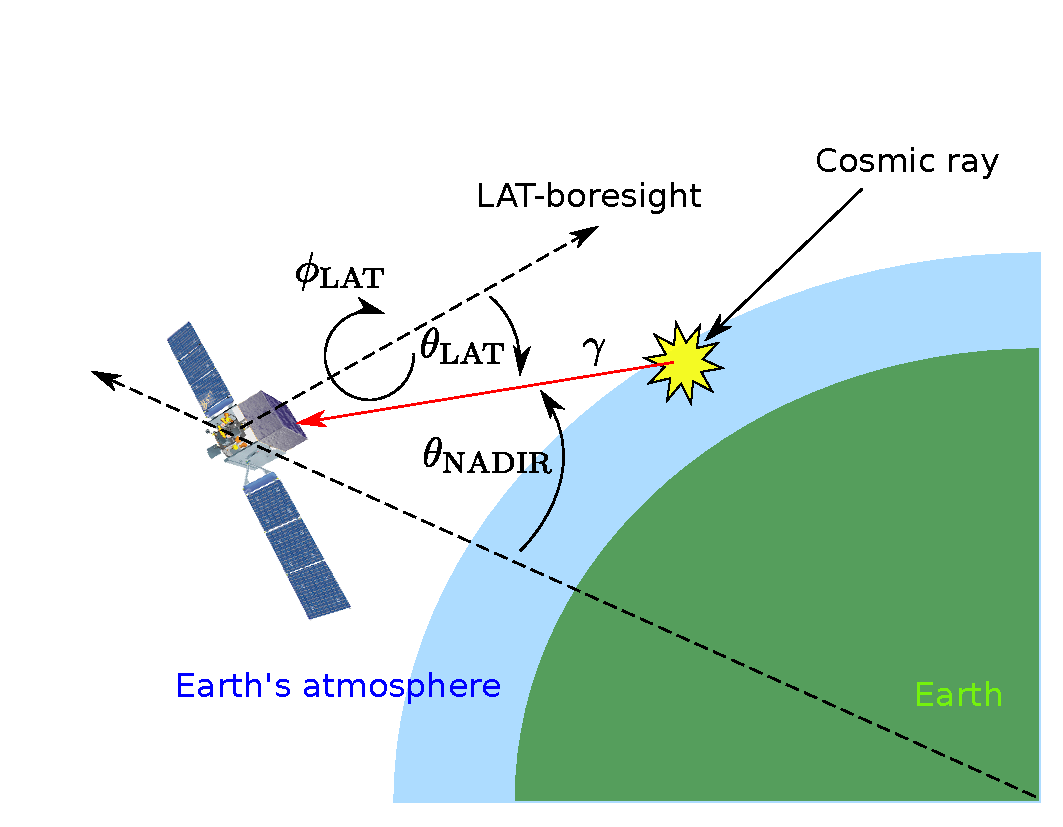
\includegraphics[width=0.7\textwidth]{img/gamma_production_schematic}
    \caption{Schematics of $\gamma$-ray production}
\end{figure}

% what is crs

\acl{CR}s are high energic particles which are produced in space by various types of acceleration mechanisms such as  supernovae, active galactic nuclei, quasars, and gamma-ray bursts. The main composition of CRs consist of 90\% protons, 8\% alpha and other heavier atoms.
The main reason that makes CRs spectrum follow power law function in rigidity is that the acceleration mechanism process was dominated in Lorenzian interaction which has a characeteristic spectral index.
\par CR spectrum has various spectral indices at different energies, depending on the types of sources which can accelerate CRs to a certain energy range as shown in Figure 2.1\cite{Swordy2001}.

\begin{figure}[h!]
\centering
  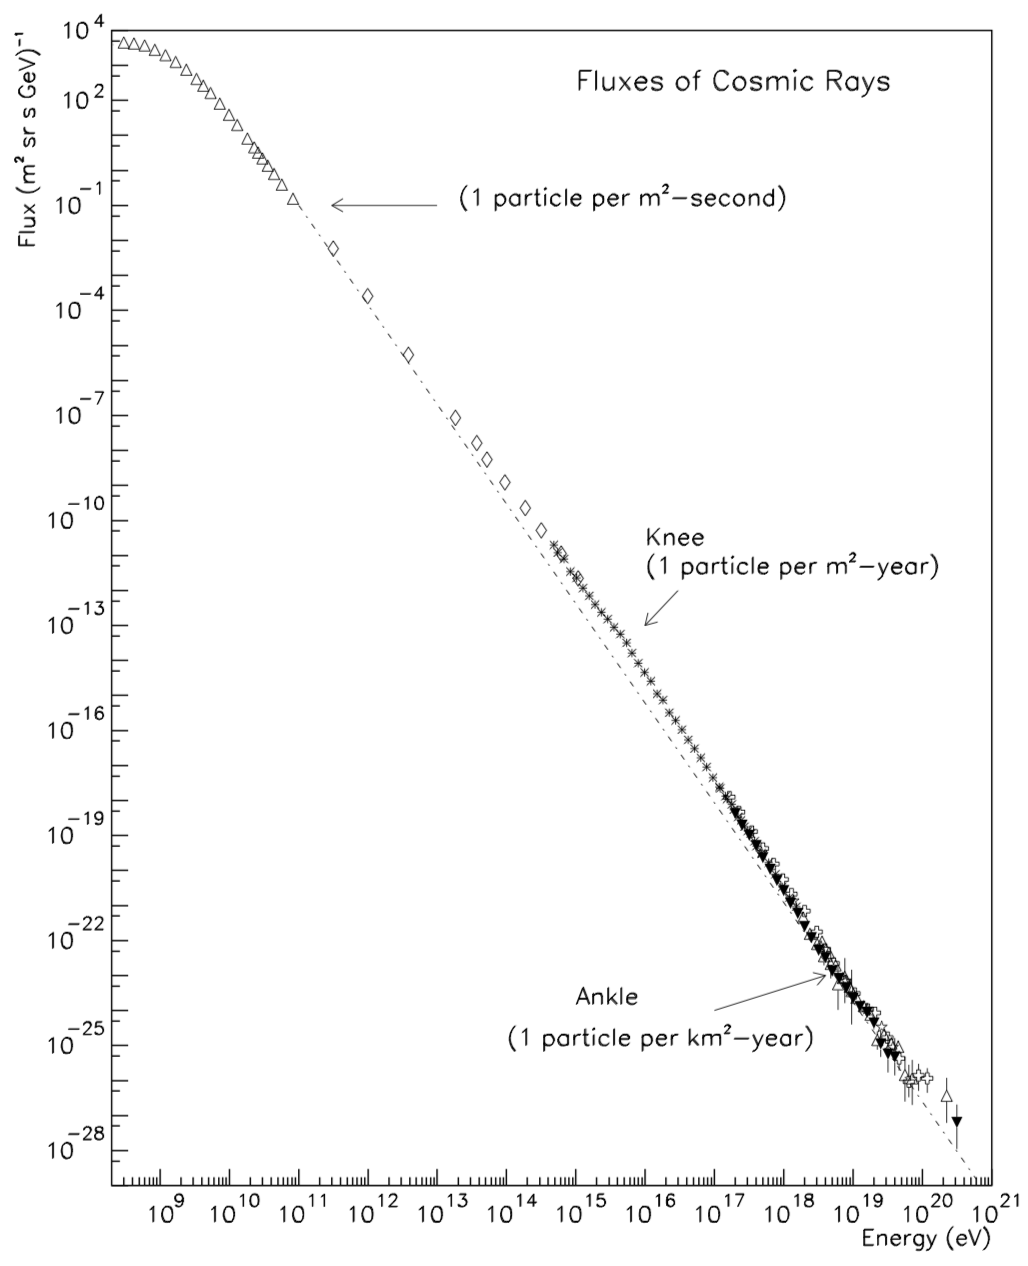
\includegraphics[width=0.6\textwidth]{img/Swordy}
  \caption{Main features of cosmic rays spectrum}
\end{figure}

% g-ray can be produced from interaction p-air 
\par The motivation why we use $\gamma$-ray as a secondary product for investigate incident proton spectrum is that Earth limb's $\gamma$-ray relatively brigher than the sky due to collision from CRs in energy range 100 MeV and 1 TeV which consistent with our study \cite{Warit2009} as the demonstration in Figure 2.2.

\par Previous work has been performed using Pass 7 version data \cite{FermiPass7} and found an energy break point around 300 GeV with a significance of about 2$\sigma$ \cite{previouswork}. This result is consistent with direct measurements from \cite{AMS-02,PAMELA}.


%==========================
%     Fermi LAT
%==========================
\newpage
\section{\acl{Fermi-LAT} }
% introduce telescope before
Gamma-ray Large Area Space Telescope (GLAST) could be informally called \acf{Fermi-LAT}. The mission is to collect data of particles from multiple phenomena such as active galaxy nuclei (AGN), pulsars and other high energy sources.
It also attach the Gamma-ray Burst Monitor (GBM) to study gamma-ray bursts. Fermi was launched on 11 June 2008 at 16:05 UTC aboard a Delta II 7920-H rocket. Please note that the main content of this section is revised from \cite{FermiStructure}.

\subsection{Apparatus}
LAT consist with 16 layers of traker (TKR) modules, 16 calorimeter (CAL) and a parition ACD. 

\begin{figure}[h!]
  \centering
    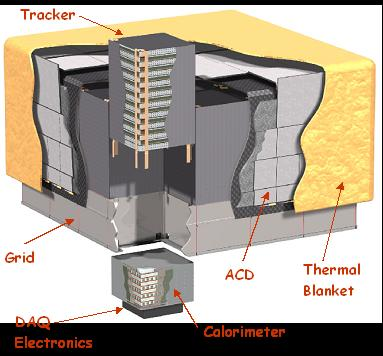
\includegraphics[width=0.5\textwidth]{img/LATStructure}
    \caption{Instrument structure : Image taken from https://fermi.gsfc.nasa.gov}
\end{figure}

\par TKR module has made from an array of silicon-strip tracking detectors (SSDs) and has 18 tracker on a horizontal planes. First 12 planes have 0.035 radiation lengths, next 4 layes contain 0.18 radiation lengths thick and the rest of it does not have any converter.
Tracking detector in each plane consist of two planar inner layer which running in x and y axis subsequently. The arrival $\gamma$-ray in LAT's field of view could produce electron-positron pair in TKR's plates.
The initial lepton pair could be determined from the recoed of conversion point in SSD planes with a power angular resolution when has a low energy.

\par Each CAL module contains 1536 CsI(Tl) crystal with an 96 crystal align in eight different orthogonal layers.
Dual PIN photodiodes also attach in each crystal which provide a great resolution in energy.

\par ACD tile contain wavelength shifting fiber by photomultiplier tubes (PMT) for redundancy. 
The tiles also are piled up in one direction.

 


\subsection{Event reconstruction}
The methodlogy of detection is to track the lepton pair product from an incident photon that collide with a conversion foils and lepton produc be traced by second inner layer of TKR.
Consequently, the limit of precision depends on energy of photon that larger than mass energy of electron-positron as well as angle resolution of TKR that getting worser and worser at larger $\theta_\text{LAT}$.
Lastly, the lepton product could be measured the energy by a high precision crystal array in CAL. The event classification also divided into various level of confident event reconstruction with a different Instrument respondse function \cite{FermiDetail,Atwood:2013rka}.


\begin{figure}[h!]
  \centering
    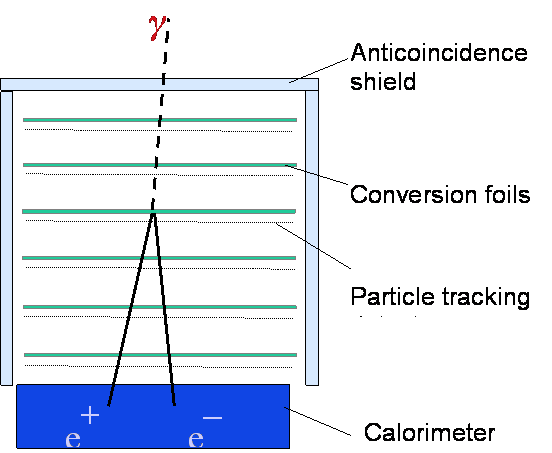
\includegraphics[width=0.5\textwidth]{img/LATMethodology}
    \caption{Schematic Structure of the LAT : Image taken from https://fermi.gsfc.nasa.gov}
  \end{figure}
 % Knowledge background

\chapter{Literature review}
\lhead{Literature review}

\chapter{Methodology}
\lhead{Methodology}

\section{Data sets}
We use only photon data with a newest version of events reconstruction (would be last version) from \acs{Fermi-LAT}
\begin{itemize}
    \item P8R2\_ULTRACLEANVETO\_V6 data from 07/08/2008 to 28/01/2015 ($\sim$7 years)
    % \item Use weekly data file from week 10 to week 399 ($\sim$ 7 years)
    \item Collect photon energy range = 10 GeV to 1 TeV
    \item $\theta_{\text{NADIR}} = 68.4^\circ - 70^\circ$(Earth’s limb) 
    \item Use $\theta_{\text{LAT}} < 70^\circ$
\end{itemize}
Note that the reasons that we use ULTRACLEANVETO type of event reconstruction are it is the cleanest reconstruction catalogue and uniform distribution of photon in the upper sky which we would use it as a background subtraction.

\section{Flux extraction}
\begin{enumerate}
    \item Reprocess photon data by taking into account
        \begin{itemize}
            \item Treat photon energy bias 3.7\% that be affected the energy range above 10 GeV
            \item Adjust limb angle due to LAT altitude shift due to detection of $\theta_{\text{Limb}}$ was tilt relatively to altitude of the spacecraft when orbit around asymmetric spherical Earth 
        \end{itemize}
    \item Construct 2D histogram in Earth's angular coordinate ($\theta_{\text{ZENITH}}$ and $\phi_{\text{EARTH}}$)
    \item Fill photon data in different energy range
    \item Calculate exposure maps which include effctive area and time that LAT field of view can glimpse area of interest
    \item Divide every single grid count map by exposure map
    \item Sum over limb region of this map then divided by solidangle and energy bin width, then fill data in $\gamma$-ray energy spectrum as the formula 3.1
    \begin{equation}
        \text{Flux}\equiv\frac{dF}{dE} = \frac{\int_{\text{Limb region}} (\text{Count map}/\text{Exposure map})}{\Delta\Omega\Delta E}
    \end{equation}
    \item Taking consider background subtraction from a average uniform background photon distribution by treating bin by bin (For more detail see Appexdix \ref{backgroundSubtract})
\end{enumerate}




\section{Interaction model}
Trail incident proton spectrum in rigidity following relation \\
\textbf{Single power law (SPL)}
\begin{equation}
\frac{dN}{dR} = R_0R^{-\gamma}
\end{equation}
\textbf{Broken power law (BPL)}
\begin{equation}
\frac{dN}{dR}=
  \begin{cases}
    R_0R^{-\gamma_1}\ :\ E < E_{\text{Break}}\\
    R_0[R(E_{\text{Break}})]^{\gamma_2-\gamma_1}R^{-\gamma_2}\ :\ E \ge E_{\text{Break}}
  \end{cases}
\end{equation}
Note that power law spectrum in energy has shown in Appendix B.

In this work, we use the scattering amplitude from hadronic collision \cite{K&Omodel} that could produce a photon particle that could be detected by \acs{Fermi-LAT}.
\begin{equation}
    \frac{dN_\gamma}{dE_\gamma} \propto \int^{E_{\text{max}}}_{E_\gamma} dE'\frac{dN_p}{dE'} \frac{d\sigma^{pp\rightarrow\gamma}(E',E_\gamma)}{dE_\gamma}
\end{equation}
\par The atmospheric composition already known well enough that mostly combined with nitrogen gas as well as oxygen molecules \cite{atmosCompos}. 
In order to get scattering amplitude from proton-proton collision we treat a crossection of single hadronic collision with a fraction of nitrogen atom which is almost equal to oxygen atom \cite{WAtwater} at relativistic level of kinetic energy.
\par In 2015, the direct measurement of Helium specrtum already reported in \cite{AMS-02Helium}. Improvement of model precision was included by taking into account incident of Helium cosmic ray particle as a first order correction and please note that we ignore other heavier atom. The derived equation relation has shown in Eq 3.3 (Derivation has done explicitly in Appendix C)

\begin{equation}
    \frac{dN_{\gamma}}{dE} \propto \sum_{E_{\text{inc,i}}}\left[\frac{E_{\text{inc,i}}}{E_{\gamma\text{,i}}}\Delta(E_{\text{inc,i}}) \right]\left[ f_{pp}\textcolor{red}{\frac{dN_\text{H}}{dE_{\text{inc,i}}}}\left\{ 1+\textcolor{olivegreen}{\frac{\sigma_{\text{HeN}}}{\sigma{pN}}}\left(\textcolor{red}{\frac{dN_{\text{H}}}{dR}}\right)^{-1} \textcolor{blue}{\frac{dN_{\text{He}}}{dR}} \frac{dR_{\text{He}}}{dR_{\text{H}}}  \right\}\right]
\end{equation}

where
\begin{itemize}
    \item Red color terms is using for \textcolor{red}{incident proton spectrum} that has form like Eq 3.4
    \item \textcolor{blue}{Use helium spectrum from AMS-02 measurement (2015)}
    \item $f_{pp}\equiv E_\gamma(d\sigma^{ij\rightarrow\gamma}/dE_\gamma)$ is a table in K$\&$O model which behave like a scattering amplitude
    that depend on the energy of incident particle
    \item Crossection \textcolor{olivegreen}{$\sigma_{\text{HeN}}/\sigma_{pN}$} at high energy ($>$ 10GeV) is quite stable ($\approx 1.6$)
\end{itemize}

\section{Optimization}

\par \textbf{Poisson likelihood function} define as Eq 3.6
\begin{equation}
    \mathcal{L} = \prod_{i=1}^{N} P_{\text{pois}}(n_{\text{i,model}}, n_{\text{i,measurement}})
\end{equation}
Since our spectrum order is in different decade, we redefined a likelihood as a log-likelihood function for numerically reason like Eq 3.7. In addition, 
\begin{equation}
    Sum = \sum_{i=1}^{N} -\log P_{\text{pois}}(n_{\text{i,model}}, n_{\text{i,measurement}})
\end{equation}


\par In order to get a best fit spectral indices, we do an optimization with a proper trial parameters for take gradient descent from Poisson loss function between model spectrum and flux from measurement as Figure 3.1


% Define block styles
\tikzstyle{decision} = [diamond, draw, fill=red!10, 
    text width=4.5em, text badly centered, node distance=3cm, inner sep=0pt]
\tikzstyle{block} = [rectangle, draw, fill=blue!10, 
    text width=7em, text centered, rounded corners, minimum height=4em]
\tikzstyle{longblock} = [rectangle, draw, fill=blue!10, 
    text width=10em, text centered, rounded corners, minimum height=4em]
\tikzstyle{line} = [draw,thick, -latex']
\tikzstyle{cloud} = [draw, ellipse,fill=red!20, node distance=3cm,
    minimum height=4em]

\begin{figure}[!h]
    \centering
    \begin{tikzpicture}[node distance = 10em, auto]
        \node [block, fill=black!10] (powerlaw) {powerlaw spectrum of proton in rigidity};
        \node [block, right of = powerlaw, node distance = 15em] (model) {$\gamma$-ray spectrum from model};
        \node [block, right of = model] (measurement) {$\gamma$-ray spectrum from measurement};
        \node [block, below left of = measurement, node distance = 12em] (pois) {Poisson likelihood function};
        \node [block, below of = powerlaw] (varyPar) {Apply gradient to parameters $\gamma$, $R_0$};
        \node [decision, below of = varyPar, fill = blue!10] (bestfit) {Best fit?};
        \node [block, right of = bestfit, node distance = 15em, fill = red!10] (return) {Return best fit parameters};

        \path [line] (powerlaw) -- node [anchor=south] {K\&O model} (model);
        \path [line] (model) -- (pois);
        \path [line] (measurement) -- (pois);
        \path [line] (pois) -- (bestfit);
        \path [line] (bestfit) -- node [anchor=east] {No} (varyPar);
        \path [line] (varyPar) -- (powerlaw);
        \path [line] (bestfit) -- node [anchor=north] {Yes} (return);
    \end{tikzpicture}
    \caption{Flow chart of optimization process}
\end{figure}




\section{Monte Carlo Simulation}
In this section, we perform a brute force method to find an error of any parameters (spectral indices and break point energy). For a \textbf{statistical error (random error)}, we rerandom a counts on each bin by poisson random generator and recalculate the flux after that optimize it as the Fig 3.1 do. The process of this algorithm has shown in Fig 3.2. We do this process as much as gaussian distribution curve looks obvious enough which our work done is roughly 2000 sampling.

\begin{figure}[h]
    \centering
    \begin{tikzpicture}[node distance = 12em, auto]
        \node [decision, fill = black!10, text width = 6em] (sampling) {While \\ sample $<$ N};
        \node [block, right of = sampling] (randStat) {Random raw count every bin by using Poisson function};
        \node [block, right of = randStat] (fluxcompute) {Calculate new $\gamma$-ray spectrum};
        \node [block, below of = fluxcompute, fill=yellow!10] (optimize) {Optimization process};
        \node [block, below of = optimize, node distance = 8em, fill = green!10] (Filled) {1D Histogram for individual parameters};
        \node [block, below of = sampling] (fitgaus) {Fit gaussian function};
        \node [block, below of = fitgaus, fill=red!10] (return) {Return value $\sigma$ of various parameters};

        % \node [block, left of = randStat]
        \path [line] (sampling) -- node [anchor=south] {Yes} (randStat);
        \path [line] (randStat) -- (fluxcompute);
        \path [line] (fluxcompute) -- (optimize);
        \path [line] (optimize) -- (sampling);
        \path [line] (sampling) -- node [anchor=west] {No} (fitgaus);
        \path [line, dashed] (optimize) -- node [anchor=east] {Fill} (Filled);
        \path [line, dashed] (Filled) -- node [anchor=south] {Send histogram information} (fitgaus);
        \path [line] (fitgaus) -- (return);
    \end{tikzpicture}
    \caption{Flow chart of Monte Carlo simulation for statistical error}
\end{figure}

\par For \textbf{total error}, we also take into account erro from instrument which is LAT that depends on energy. We exactly the same as the statistical error determination but one more thing that including to this algorithm is to pick three energy bin (10, 100, 1000 GeV) then rerandom flux in these three bin and apply a cubic spline interpolation to smooth the line for a statistical reason \cite{FermiDetail}. The deminstration of this program is shown as Fig 3.3.


\begin{figure}[h]
    \centering
    \begin{tikzpicture}[node distance = 12em, auto]
        \node [decision, fill = black!10, text width = 6em] (sampling) {While \\ sample $<$ N};
        \node [block, right of = sampling] (randStat) {Random raw count every bin by using Poisson function};
        \node [block, right of = randStat] (fluxcompute) {Calculate new $\gamma$-ray spectrum};
        \node [longblock, below of = fluxcompute] (randSys) {Pick 3 point (10 , 100 , 1000 GeV) and use gaussian random which $\sigma$ came from
        Aeff (LAT effective area) then apply cubic spline interpolation};
        \node [block, below of = randSys, fill = yellow!10] (optimize) {Optimization process};
        \node [block, below of = optimize, fill = green!10] (Filled) {1D Histogram for individual parameters};
        \node [block, below of = sampling] (fitgaus) {Fit gaussian function};
        \node [block, below of = fitgaus, fill=red!10, node distance = 15em] (return) {Return value $\sigma$ of various parameters};
        % \node [block, left of = randStat]
        \path [line] (sampling) -- node [anchor=south] {Yes} (randStat);
        \path [line] (randStat) -- (fluxcompute);
        \path [line] (fluxcompute) -- (randSys);
        \path [line] (randSys) -- (optimize);
        \path [line] (optimize) -- (sampling);
        \path [line] (sampling) -- node [anchor=west] {No} (fitgaus);
        \path [line, dashed] (optimize) -- node [anchor=west] {Fill} (Filled);
        \path [line, dashed] (Filled) -- node [anchor=south] {Send histogram information} (fitgaus);
        \path [line] (fitgaus) -- (return);
    \end{tikzpicture}
    \caption{Flow chart of Monte Carlo simulation for total error}
\end{figure}

\section{\acf{lrt}}
In order to determine significant level between null model and alternative model, we use Wilk's theorem \cite{Wilks1938}.
Basically, this method is to regard a given likelihood
\begin{equation}
    \mathcal{L} \equiv \prod_{\alpha=1}^n f(x_\alpha, \theta_1, \theta_2, ..., \theta_h)
\end{equation}
where 
\begin{itemize}
    \item $x_\alpha$ is represent a variant from model and data
    \item $\theta_i$ is a degree of freedom (DOF)
\end{itemize}
The explicit declaration with an obvious method to implement has been proved in \cite{Huelsenbeck} as the Equation 3.9
\begin{equation}
    \text{LRT} = -2\ln\left(\frac{\mathcal{L}_\text{null}}{\mathcal{L}_\text{alternative}}\right)
\end{equation} % Methodology

\chapter{Results and discussion}
\lhead{Results and discussion}


\section{Limb's angle correction}
Since we already take into account $\theta_\text{ZENITH}$ shifted due to Earth's radial asymmetry, we should see the count distribution versus $\theta_\text{NADIR}$ with lesser standard deviation as Figure 4.1.

\begin{figure}[h!]
    \centering
      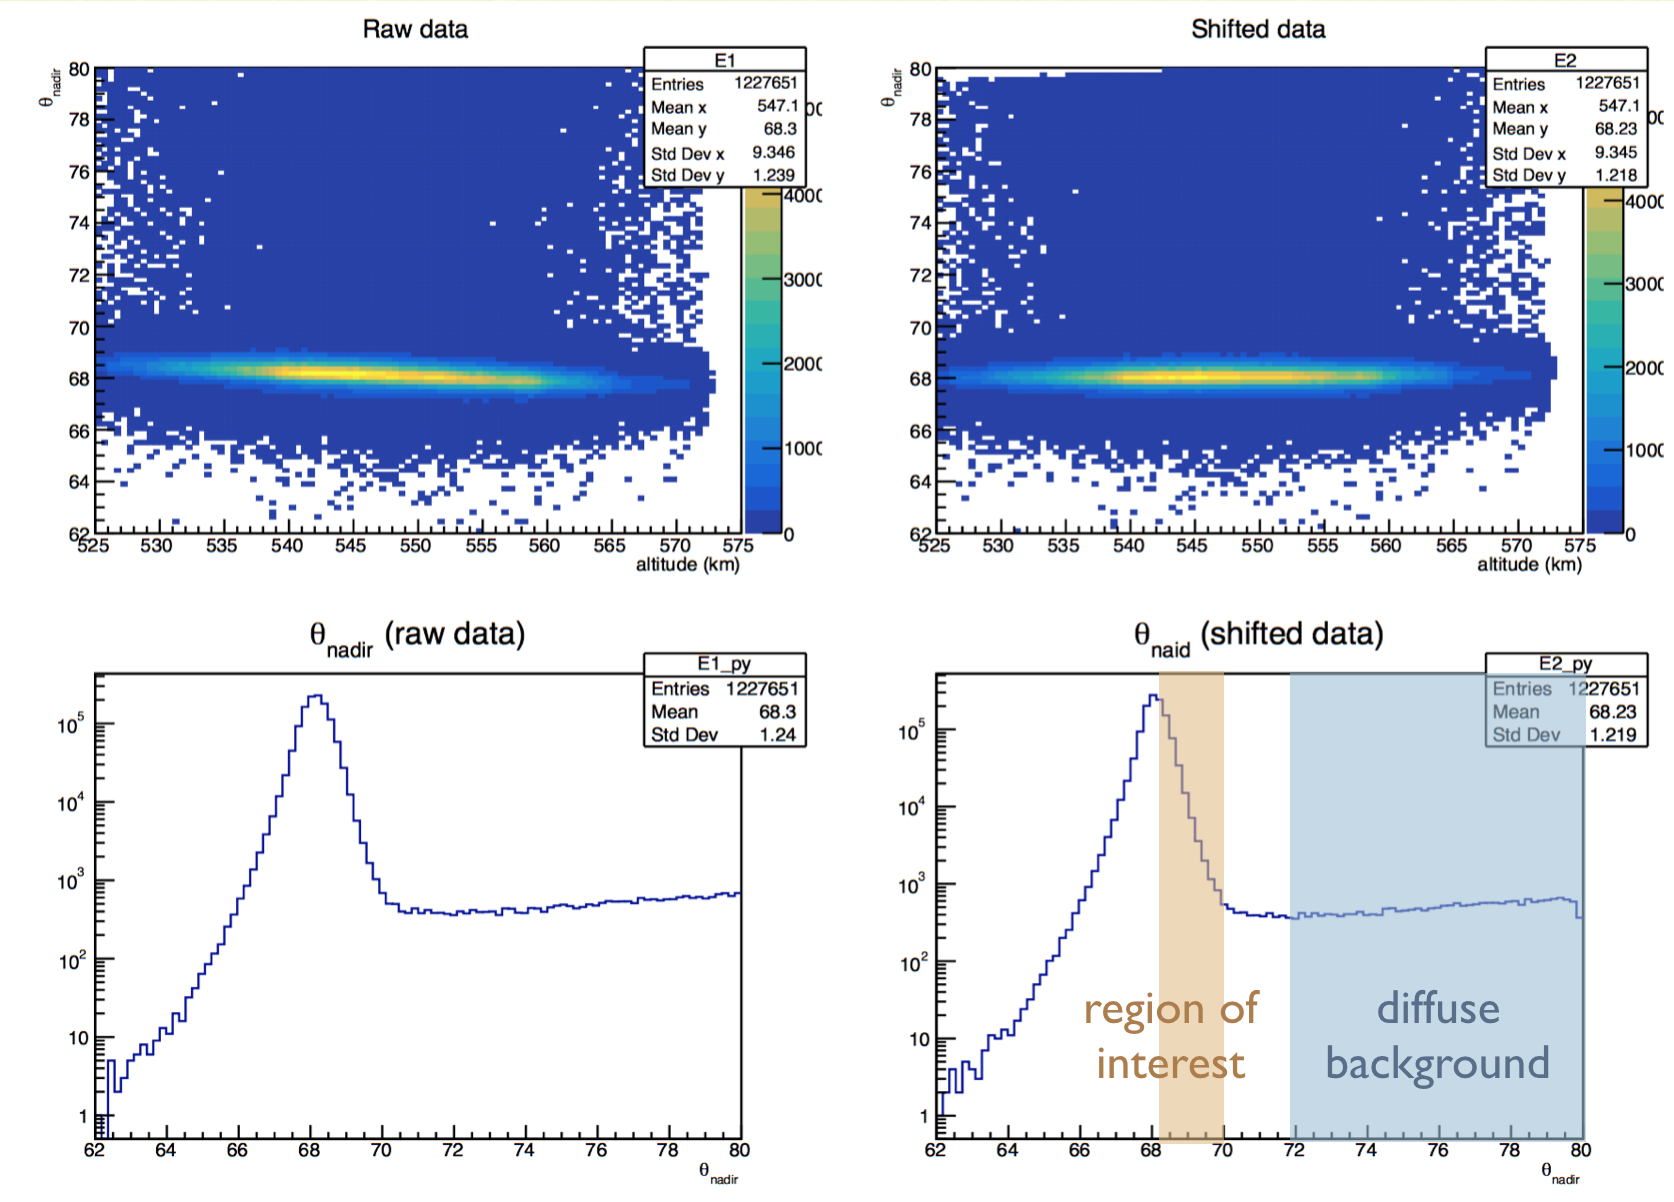
\includegraphics[width=\textwidth]{img/LATShifted}
      \caption{Distribution of nadir angle before and after altitude correction}
\end{figure}

%%%%%%%%%%%%%%%%%%%%%%%%%%%%%%%
%%%%%  gamma-ray spectrum   %%%
%%%%%%%%%%%%%%%%%%%%%%%%%%%%%%%
\section{$\gamma$-ray spectrum}
In this section, we provide an example of various map that we use in Earth's angular coordinate. Please note that we pick only 4 various energy bin to demenstrate by starting with Figure 4.2 for fill a raw event in the map. 
In order to get an exposure map, we have to dive deep to spacecraft log file to simulate field of view of LAT for count time in each grid on geologic's angular coordinate as well as regard effective area of LAT in different angle as shown in Figure 4.3. Intensity map of photon has a characteristics identification of west and north side like in Fig 4.4, it is obvious to see that west side has higher density than east side because geomagnetic cutoff rigidity when this effect dominated in a lower rigidity.
Finally, $\gamma$-ray spectrum as in Figure 4.5 could be computed from count map and exposure map with a calculation of Eq (3.1).
%%% show any map & flux
\begin{figure}[h!]
    \begin{tikzpicture}
    \node (0,0) {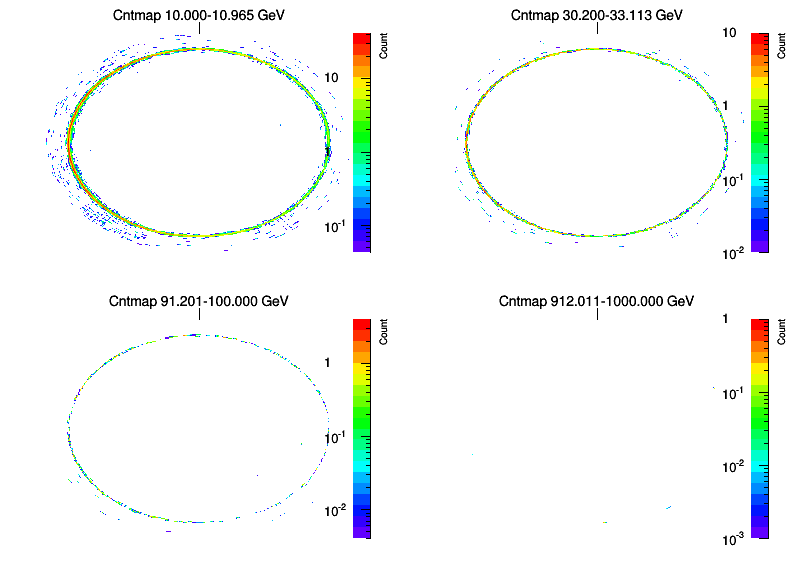
\includegraphics[width=\textwidth]{img/cntmapAfterCut}};
    \node [opacity=0.2] (0,0) {\rotatebox{45}{\scalebox{3.0}{\textcolor{red}{preliminary}}}};
    \end{tikzpicture}
    \caption{Count map}
\end{figure}


\begin{figure}[h!]
    \begin{tikzpicture}
    \node (0,0) {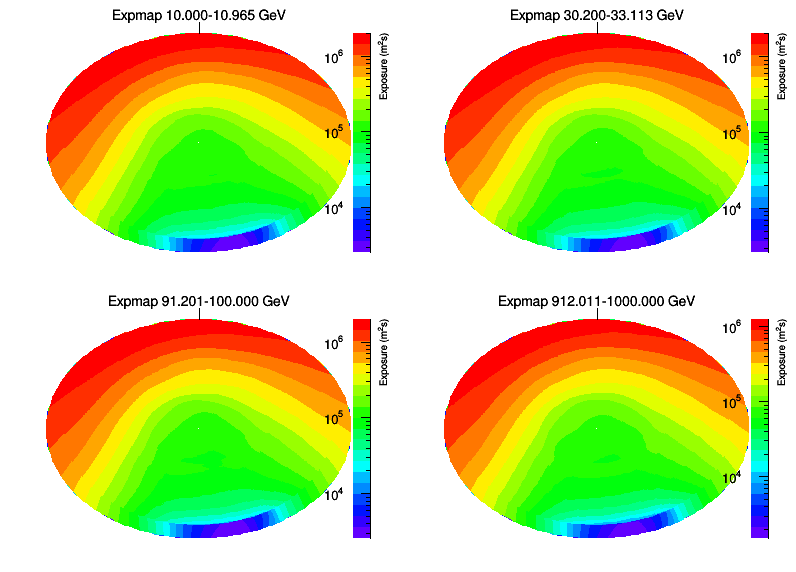
\includegraphics[width=\textwidth]{img/expmapAfterCut}};
    \node [opacity=0.2] (0,0) {\rotatebox{45}{\scalebox{3.0}{\textcolor{red}{preliminary}}}};
    \end{tikzpicture}
    \caption{Exposure map}
\end{figure}

\begin{figure}[h!]
    \begin{tikzpicture}
    \node (0,0) {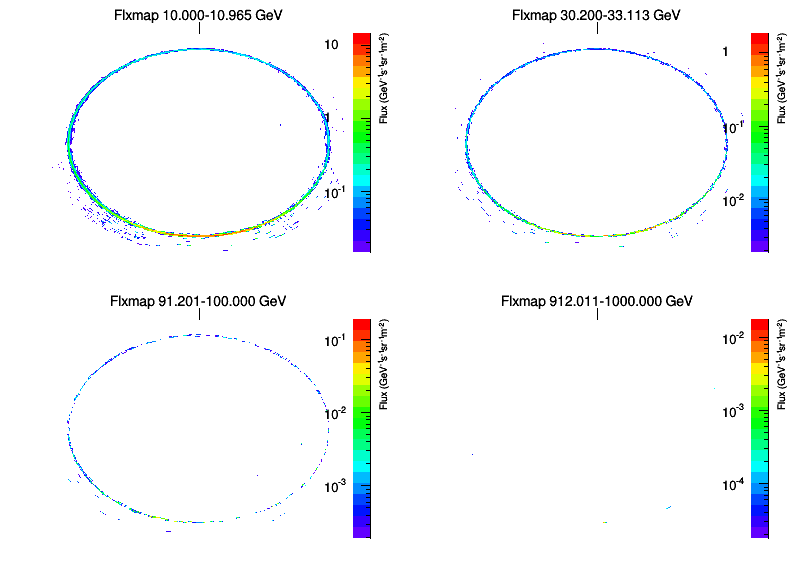
\includegraphics[width=\textwidth]{img/flxmapAfterCut}};
    \node [opacity=0.2] (0,0) {\rotatebox{45}{\scalebox{3.0}{\textcolor{red}{preliminary}}}};
    \end{tikzpicture}
    \caption{Flux map}
\end{figure}
 
\begin{figure}[h!]
    \begin{tikzpicture}
    \node (0,0) {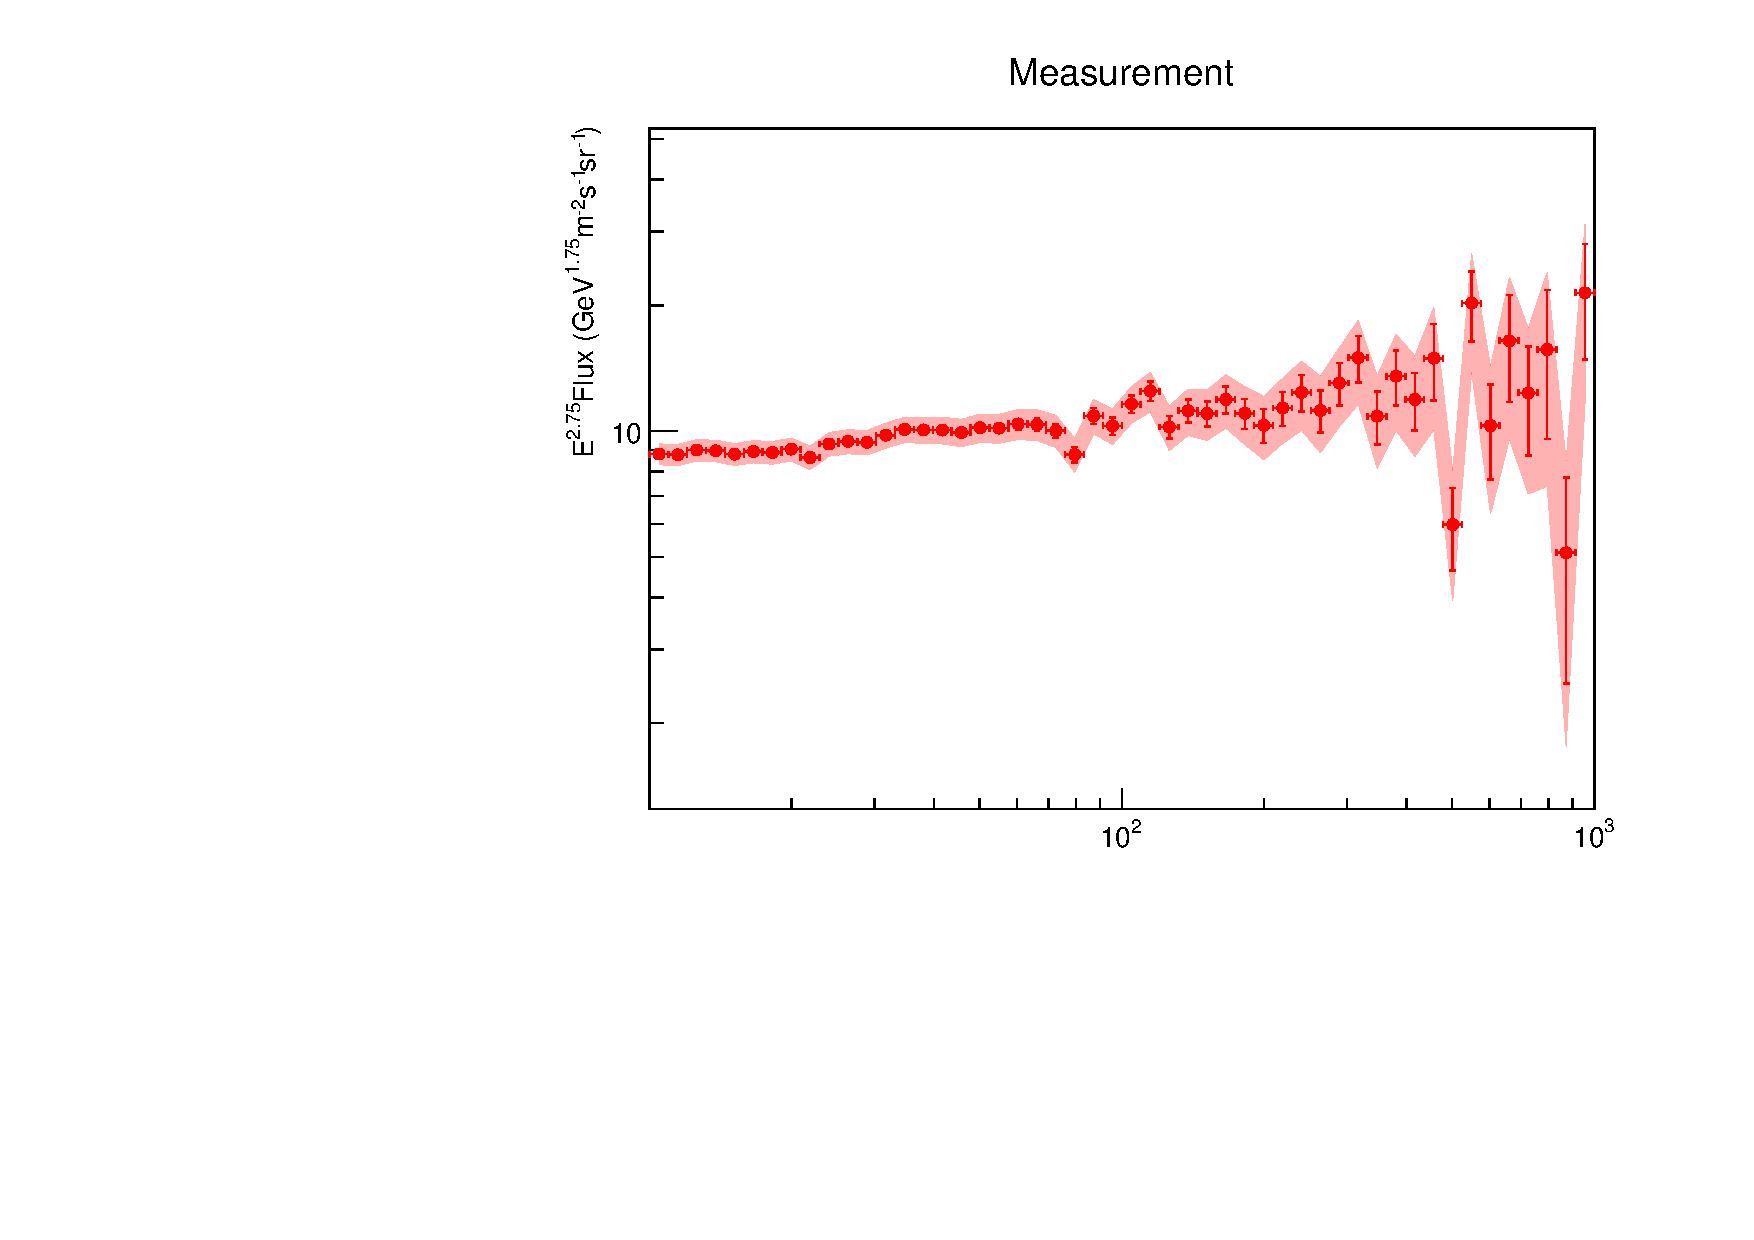
\includegraphics[width=\textwidth]{img/FluxFromExposure}};
    \node [opacity=0.2] (0,0) {\rotatebox{45}{\scalebox{3.0}{\textcolor{red}{preliminary}}}};
    \node [opacity=1.0] at (4.9,-4.7) {E (GeV)};
    \end{tikzpicture}
    \caption{$\gamma$-ray energy spectrum}
\end{figure}


%%%%%%%%%%%%%%%%%%%%%%%%%%%%%%%%%%%%%%%
%%%%%  Power law from measurement   %%%
%%%%%%%%%%%%%%%%%%%%%%%%%%%%%%%%%%%%%%%
\clearpage
\section{Power law from indirect measurement}
The measured parameters of SPL and BPL model has been calculated from optimization process has shown in Table 4.1 and we found that BPL fits better than SPL with a significant level of $3.3\sigma$. 
Note that statistical and total (including systematic error) error computed from Monte Carlo Simulation
The demonstration of $\gamma$-ray from model and measurement also represent in Figure 4.6 as well as Figure 4.7 show a renormalized proton spectrum from this work (indirect measurement) compare with other direct measurement.
% table of SPL & BPl parameters with significant ref from Wilk's theorem
\begin{table}[h!]
    \begin{tabular}{l | c | c | c}
      Best fits & $\gamma_1$ & $\gamma_2$ & $E_{\text{Break}}$ (GeV) \\
      \hline \hline
      Single Power Law (SPL) & 2.68 $\pm$ 0.01(0.03) & - & -  \\
      Broken Power Law (BPL) & 2.84 $\pm$ 0.04(0.06) & 2.64 $\pm$ 0.04(0.17) & 328 $\pm$ 151(267)
    \end{tabular}
    \caption{Optimization results : \\ statistical error and total error has shown in table subsequently}
\end{table}

% gmr spectrum
\begin{figure}[h!]
    \begin{tikzpicture}
    \node (0,0) {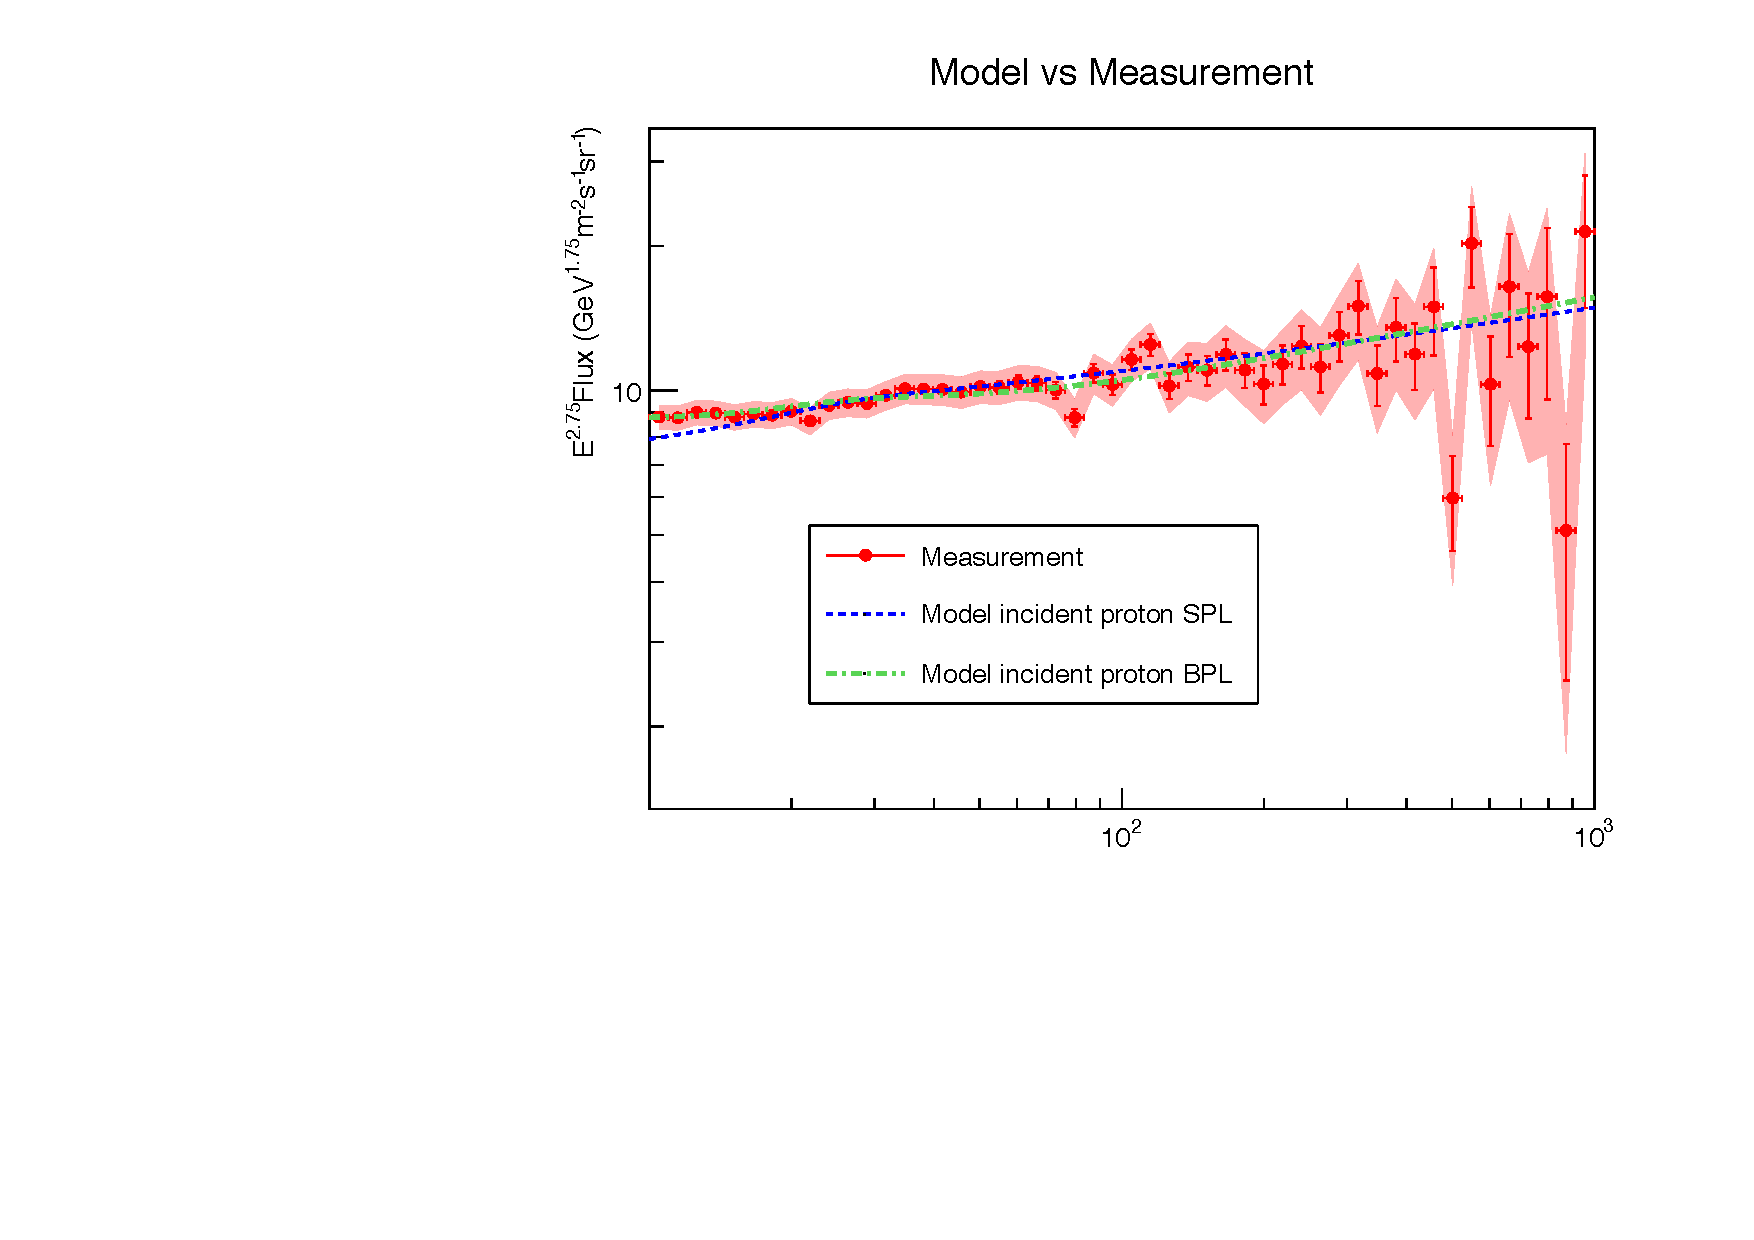
\includegraphics[width=\textwidth]{img/ModelVSMeasurement}};
    \node [opacity=0.2] (0,0) {\rotatebox{45}{\scalebox{3.0}{\textcolor{red}{preliminary}}}};
    \node [opacity=1.0] at (4.9,-4.7) {E (GeV)};
    \end{tikzpicture}
    \caption{$\gamma$-ray spectrum from model and measurement}
\end{figure}

% proton spectrum
\begin{figure}[h!]
    \begin{tikzpicture}
    \node (0,0) {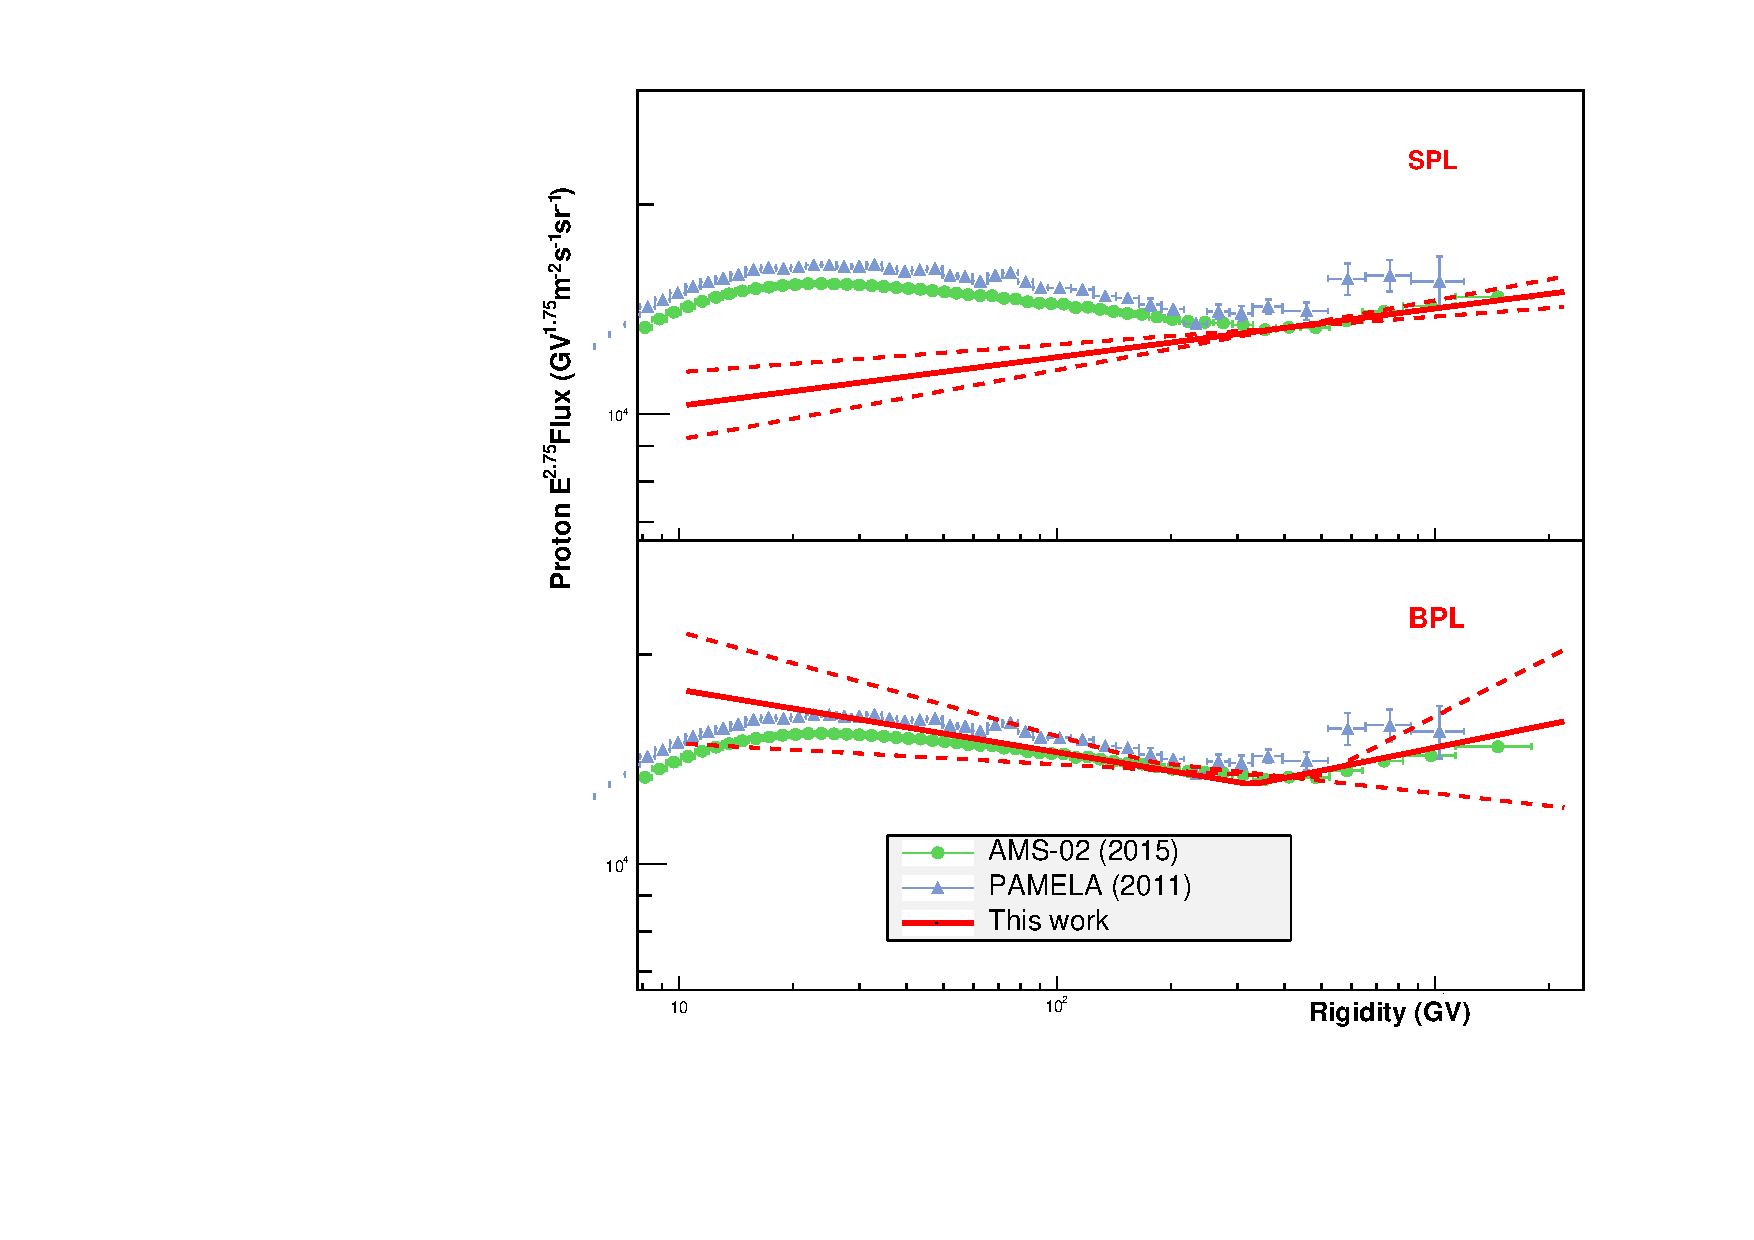
\includegraphics[width=\textwidth]{img/ProtonSpectrumModelMeasurement}};
    \node [opacity=0.2] (0,0) {\rotatebox{45}{\scalebox{3.0}{\textcolor{red}{preliminary}}}};
    \end{tikzpicture}
    \caption{Proton spectrum from model and other direct measurements}
\end{figure}
 % Results and discussion

\chapter{Conclusion}
\lhead{Conclusion}

The result of this work put weight on the previous study \cite{previouswork} that we could take a benefit of brightness $\gamma$-ray from Earth's high atmosphere to indirectly observe cosmic ray spectrum which cause this luminous. 
In this study, we perform an indirect measurement with a newest \acs{Fermi-LAT}'s reconstruction event (Pass8) with the same model and modify Helium spectrum by using AMS-02 instead of PAMELA due to it has more precise proton spectrum. To sum up, we found that there is an energy break point around 328 GeV with a significant level of 3.3$\sigma$ which agree with other direct measurement.
Even though we have found better of BPL than SPL, but we still need the significant more than 5$\sigma$ to strongly comfirm a drastic change of proton spectrum in order of hundren GeV which would be the future work. % Conclusion

%\input{Chapters/Chapter6} % Results and Discussion

%\input{Chapters/Chapter7} % Conclusion

%% ----------------------------------------------------------------
% Now begin the Appendices, including them as separate files
\lhead{}

\addtocontents{toc}{\vspace{2em}} % Add a gap in the Contents, for aesthetics

\appendix % Cue to tell LaTeX that the following 'chapters' are Appendices

\chapter{Why we can directly subtract a background photon}\label{backgroundSubtract}

\begin{figure}[h!]
    \centering
      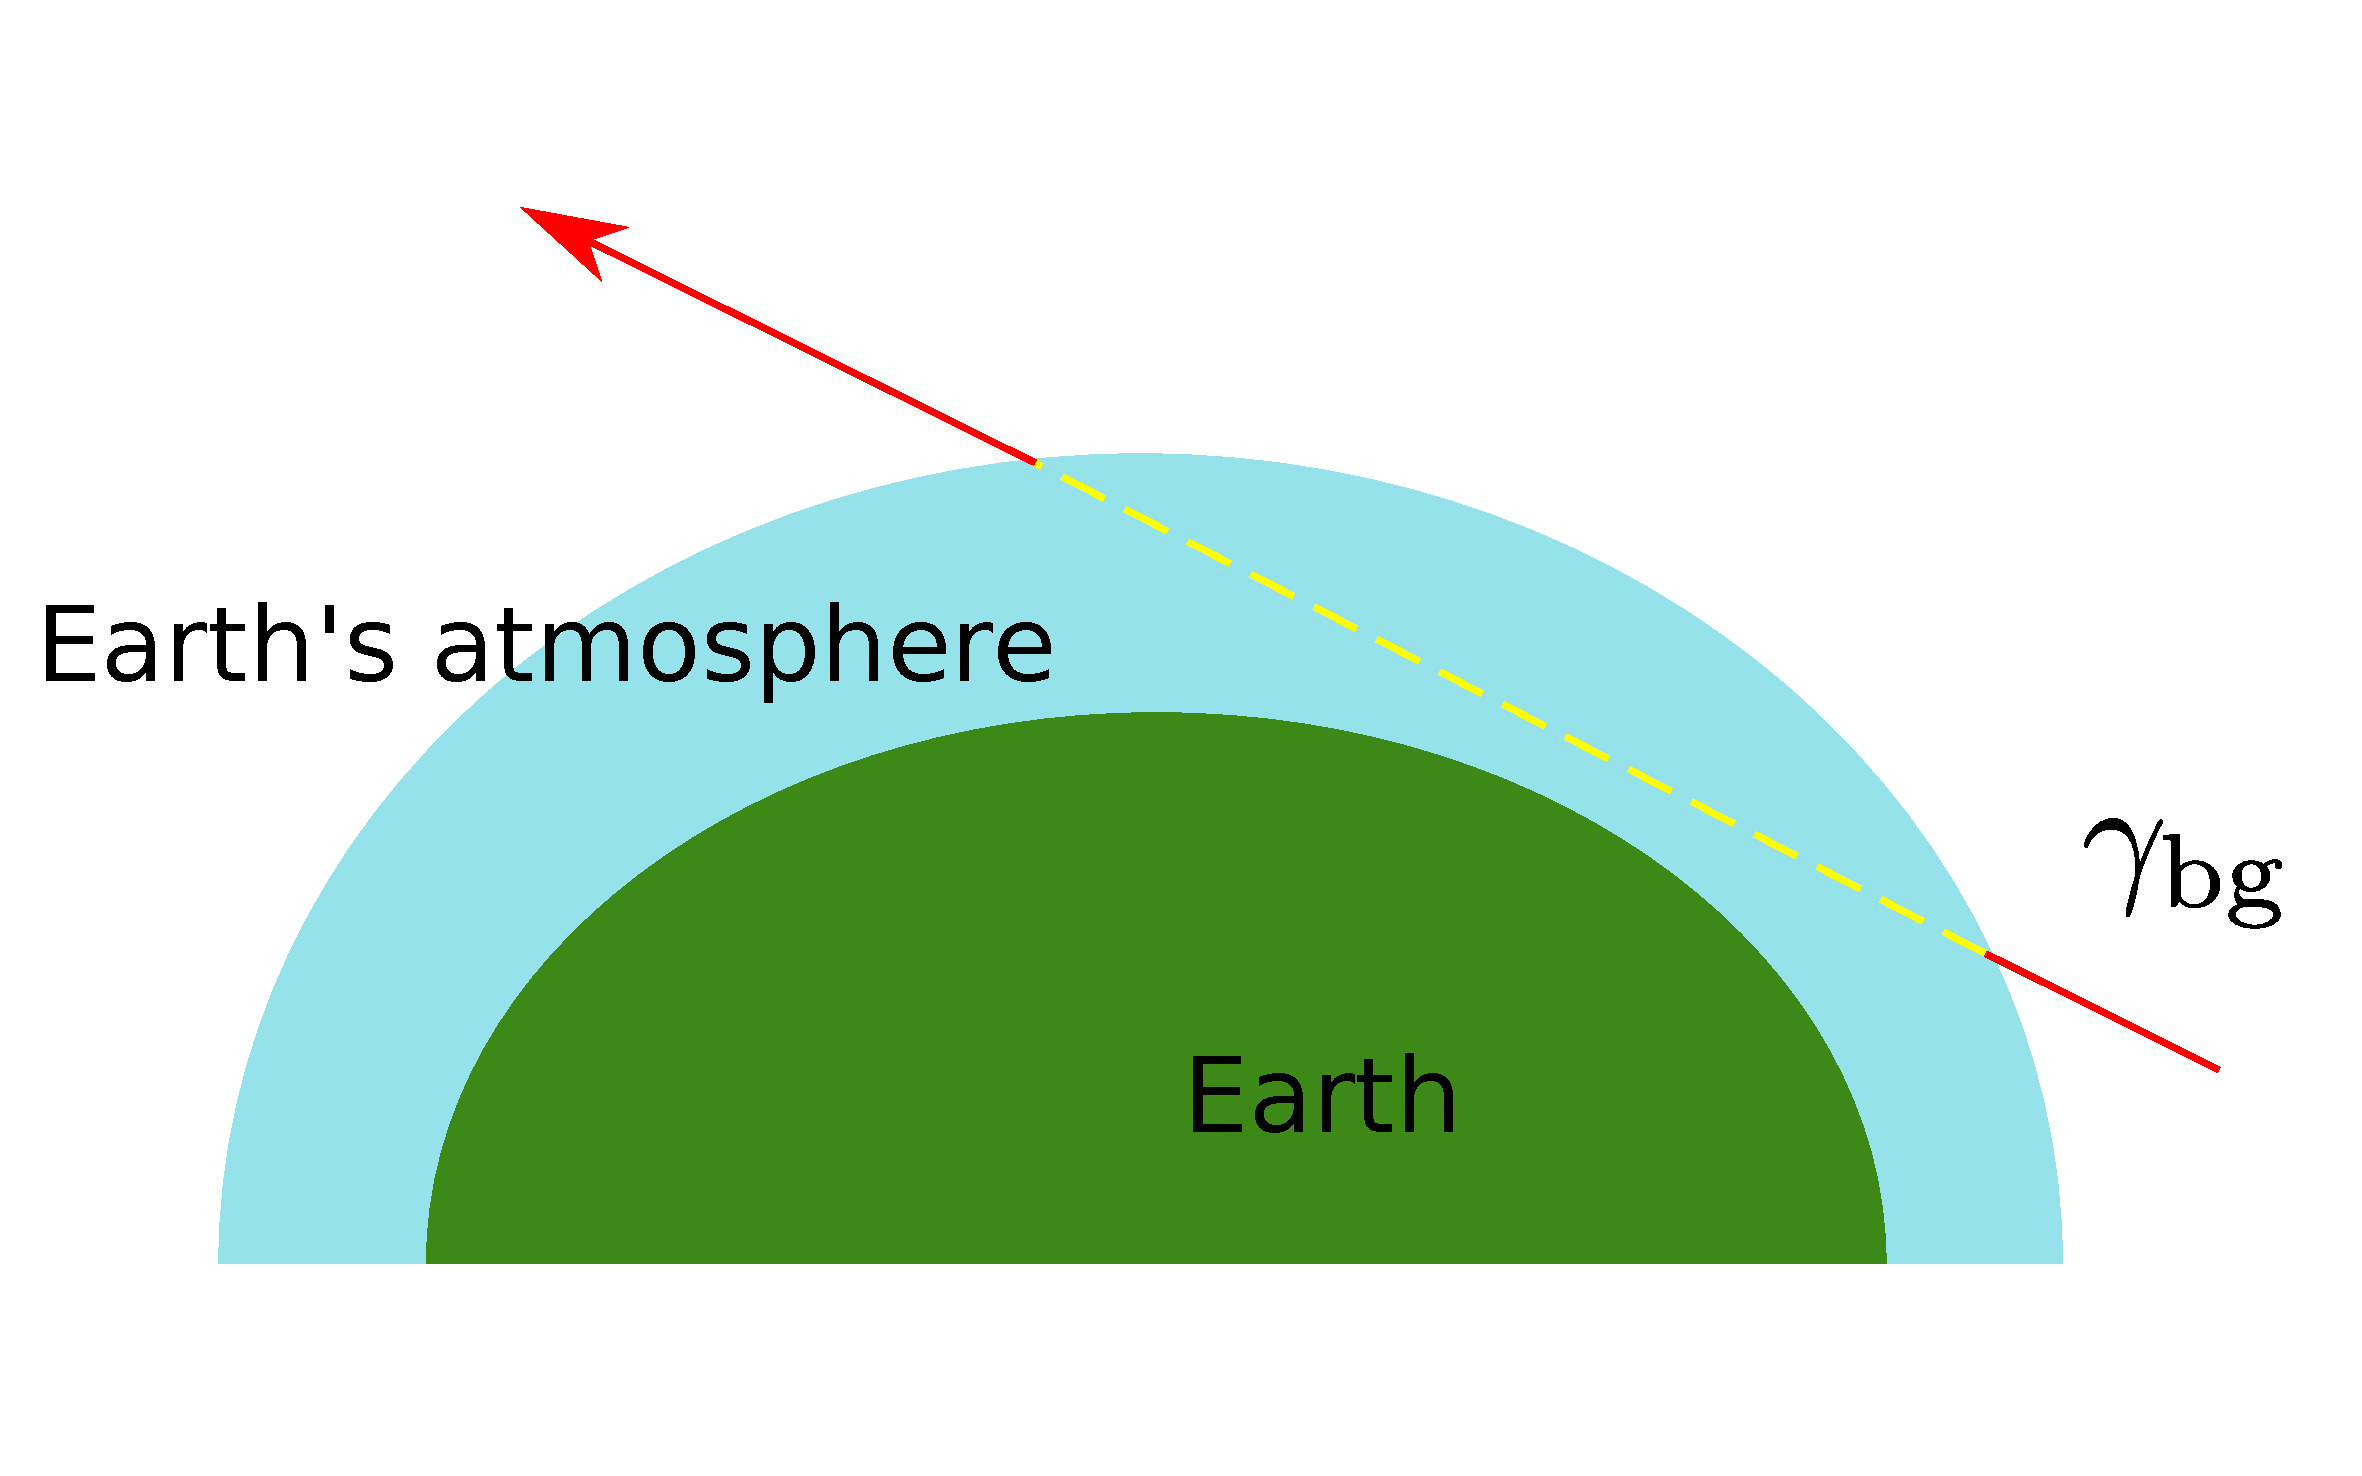
\includegraphics[width=0.7\textwidth]{img/backgroundSubtract}
      \caption{Schematics of $\gamma$-ray propagation from diffusive background}
\end{figure}

Assume Probability of collision with assume ultrarelativistic limit approached to classical concept below
\begin{equation}
    N \equiv N_0 e^{-n\sigma x}
\end{equation}
when
\begin{itemize}
    \item $n$ is a density of air
    \item $\sigma$ is a crossection
    \item $x$ is a propagation length
\end{itemize}
From using crossection data from XCOM:NIST(2010) \cite{XCOMNIST}, we found that collision probability of $\gamma$-ray with nitrogen atom and oxygen atom very similar in energy range of our interest.
If we consider in worse case scenario( longest path and highest density that could happen in atmosphere), we found a passing possibility approach to one more than third order. To sum up, we could straightforwardly remove a background by taking average diffusive background per unit of angle before to apply.


	% Appendix Title

\chapter{Power law in energy}

\textbf{Single power law (SPL)}
\begin{equation}
\frac{dN}{dE} = N_0[E_k(E_k+2m_p)]^{-\gamma/2} \left(\frac{E_k+m_p}{\sqrt{E_k(E_k+2m_p)}}\right)
\end{equation}
\textbf{Broken power law (BPL)}
\begin{equation}
\frac{dN}{dE}=
  \begin{cases}
    N_0[E_k(E_k+2m_p)]^{-\gamma_1/2} \left(\frac{E_k+m_p}{\sqrt{E_k(E_k+2m_p)}}\right)\ :\ E < E_{\text{Break}}\\
    N_0[E_b(E_b+2m_p)]^{(\gamma_2-\gamma_1)/2}[E_k(E_k+2m_p)]^{-\gamma_2/2} \left(\frac{E_k+m_p}{\sqrt{E_k(E_k+2m_p)}}\right)\\ :\ E \ge E_{\text{Break}}
  \end{cases}
\end{equation}

 % Appendix Title

\chapter{Derivation of interaction model}\label{derivationModel}

Since we know the relation of $\gamma$-ray spectrum from incident proton spectrum collide with a nitrogen atom as

\begin{equation}
    \frac{dN_\gamma}{dE_\gamma} \propto \int^{E_{\text{max}}}_{E_\gamma} dE'\frac{dN_p}{dE'} \frac{d\sigma^{pN\rightarrow\gamma}(E',E_\gamma)}{dE_\gamma}
\end{equation}

Change to discrete form

\begin{equation}
    \frac{dN_\gamma}{dE_\gamma} \propto \sum_{E_\gamma}^{E_\text{max}} \frac{E_p}{E_\gamma}\Delta(\ln E')E_\gamma\frac{d\sigma^{pN\rightarrow\gamma}}{dE_\gamma}\frac{dN_p}{dE'}
\end{equation}

Add first term correction for Helium collision and define $f_{pp}\equiv E_\gamma(d\sigma^{ij\rightarrow\gamma}/dE_\gamma)$ which came from K\&O model

\begin{equation}
\begin{split}
    \frac{dN_\gamma}{dE_\gamma} &\propto \sum_{E_\text{CR}=E_\gamma}^{E_\text{max}}\frac{E_\text{CR}}{E_\gamma}\Delta(\ln E_\text{CR})\left[ E_\gamma\frac{d\sigma^{pN\rightarrow\gamma}}{dE_\gamma}\left(\frac{dN_p}{dE_\text{CR}}\right) + E_\gamma\frac{d\sigma^{HeN\rightarrow\gamma}}{dE_\gamma}\left(\frac{dN_{He}}{dE_\text{CR}}\right) \right] \\
    &\propto \sum_{E_\text{CR}=E_\gamma}^{E_\text{max}} \left[ \frac{E_\text{CR}}{E_\gamma}\Delta(\ln E_\text{CR}) \right]\left[ f_{pp}\frac{dN_H}{dE} \left\{ 1+ \frac{\sigma_{\text{HeN}}}{\sigma_\text{pN}}\left(\frac{dN_\text{H}}{dR} \right)^{-1}\frac{dN_\text{He}}{dR}\frac{dR_\text{He}}{dR_H}\right\}\right]
\end{split}
\end{equation}

In our case, we use the fraction relation of crossection between different atom number with a limit of relativistics as \cite{WAtwater}, we have found $\sigma_{\text{HeN}}/\sigma_\text{pN} \approx 1.77$
\par Lastly, term $dR_\text{He}/dR_\text{H} = 4$ because the relativistic energy mass relation fraction of rigidity between Helium that approximately heavier than proton 4 times.
 % Appendix Title

\addtocontents{toc}{\vspace{2em}}  % Add a gap in the Contents, for aesthetics
\backmatter

%% ----------------------------------------------------------------
\label{Bibliography}
\lhead{\emph{Bibliography}}  % Change the left side page header to "Bibliography"
\bibliographystyle{unsrtnat}  % Use the "unsrtnat" BibTeX style for formatting the Bibliography
% \bibliographystyle{apsrev} % natbib-compatible style for Physical Review journals


\bibliography{Bibliography}  % The references (bibliography) information are stored in the file named "Bibliography.bib"

\end{document}  % The End
%% ----------------------------------------------------------------